\documentclass{beamer}

\usefonttheme{professionalfonts} % using non standard fonts for beamer
\usefonttheme{serif} % default family is serif

\usepackage{enumitem}
\setitemize{label=\usebeamerfont*{itemize item}%
  \usebeamercolor[fg]{itemize item}
  \usebeamertemplate{itemize item}}

\usepackage{hyperref}
\usepackage{booktabs}
\usepackage{xfp}
\usepackage{graphicx}
\def\Put(#1,#2)#3{\leavevmode\makebox(0,0){\put(#1,#2){#3}}}
\usepackage{colortbl}
\usepackage{tikz}
\usepackage{amssymb}
\usepackage{enumerate}
\usepackage{arydshln}
\usepackage{algorithm}
\usepackage{algpseudocode}
\usepackage{subcaption} %to have subfigures available

\usepackage[absolute,overlay]{textpos}

\colorlet{lightred}{red!25}
\colorlet{lightgreen}{green!25}
\beamertemplatenavigationsymbolsempty

\newcommand\blfootnote[1]{%
  \begingroup
  \renewcommand\thefootnote{}\footnote{#1}%
  \addtocounter{footnote}{-1}%
  \endgroup
}

\makeatletter

%% Textclass specific LaTeX commands.
\newcommand\makebeamertitle{\frame{\maketitle}}%
\AtBeginDocument{%
  \let\origtableofcontents=\tableofcontents
  \def\tableofcontents{\@ifnextchar[{\origtableofcontents}{\gobbletableofcontents}}
  \def\gobbletableofcontents#1{\origtableofcontents}
}
%% User specified LaTeX commands.
\usetheme{Malmoe}
\useoutertheme{infolines}
\addtobeamertemplate{headline}{}{\vskip2pt}
\setbeamercovered{transparent}

\title[PFlock report]{PFLOCK Report}
\author[AC]{Andres Calderon}
\institute[UCR]{University of California, Riverside}
\makeatother

%%%%%%%%%%%%%%%%%%%%%%%%%%%%%%%%%%%%%%
%% Main document
%%%%%%%%%%%%%%%%%%%%%%%%%%%%%%%%%%%%%%
\begin{document}
\makebeamertitle
\newif\iflattersubsect

\AtBeginSection[] {
    \begin{frame}<beamer>
    \frametitle{Outline} 
    \tableofcontents[currentsection]  
    \end{frame}
    \lattersubsectfalse
}

\AtBeginSubsection[] {
    \begin{frame}<beamer>
    \frametitle{Outline} 
    \tableofcontents[currentsubsection]  
    \end{frame}
}

%%%%%%%%%%%%%%%%%%%%%%%%%%%%%%%%%%%%%%%%%%%
%%% Finer quadtree
%%%%%%%%%%%%%%%%%%%%%%%%%%%%%%%%%%%%%%%%%%%

\begin{frame}{Uniform study area...}
    \begin{itemize}
        \item Uniform random generator\footnote{\href{https://dl.acm.org/doi/10.1145/3397536.3422351}{SpiderWeb: A Spatial Data Generator on the Web}}...
        \item Number of points: 25K 50K 75K 100K...
        \item Uniform distributed over a square of 1 unit...
        \item Performace evaluated by different quadtree capacities (100, 200 and 300 points per cell)...
    \end{itemize}
\end{frame}

\begin{frame}{Uniform study area...}
    \centering
    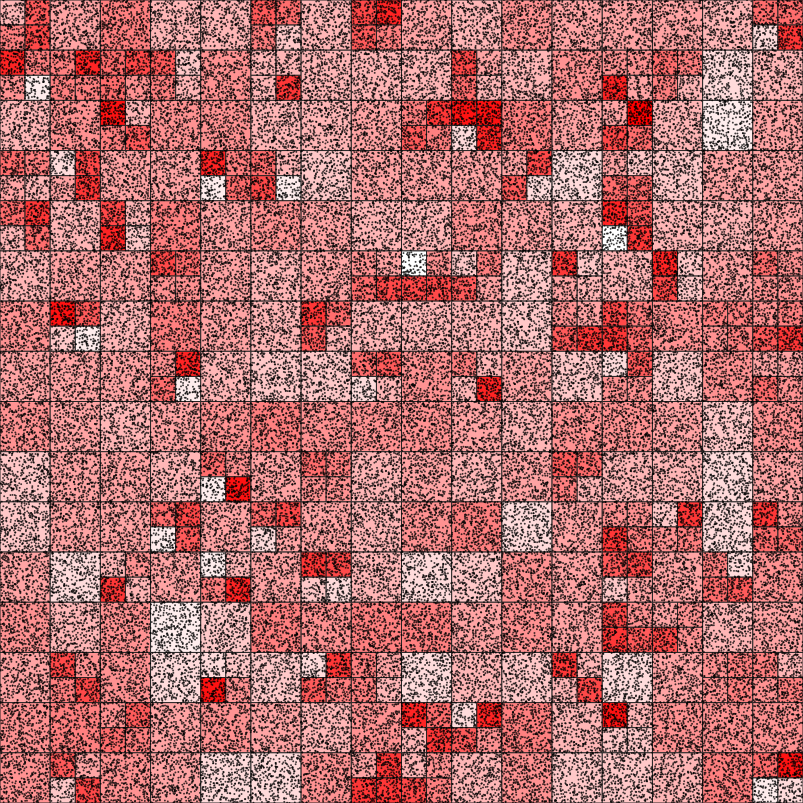
\includegraphics[width=0.60\textwidth]{figures/uniform_study_area}
\end{frame}

\begin{frame}{Performance [Datasets vs Capacity vs Epsilon]...}
    \centering
    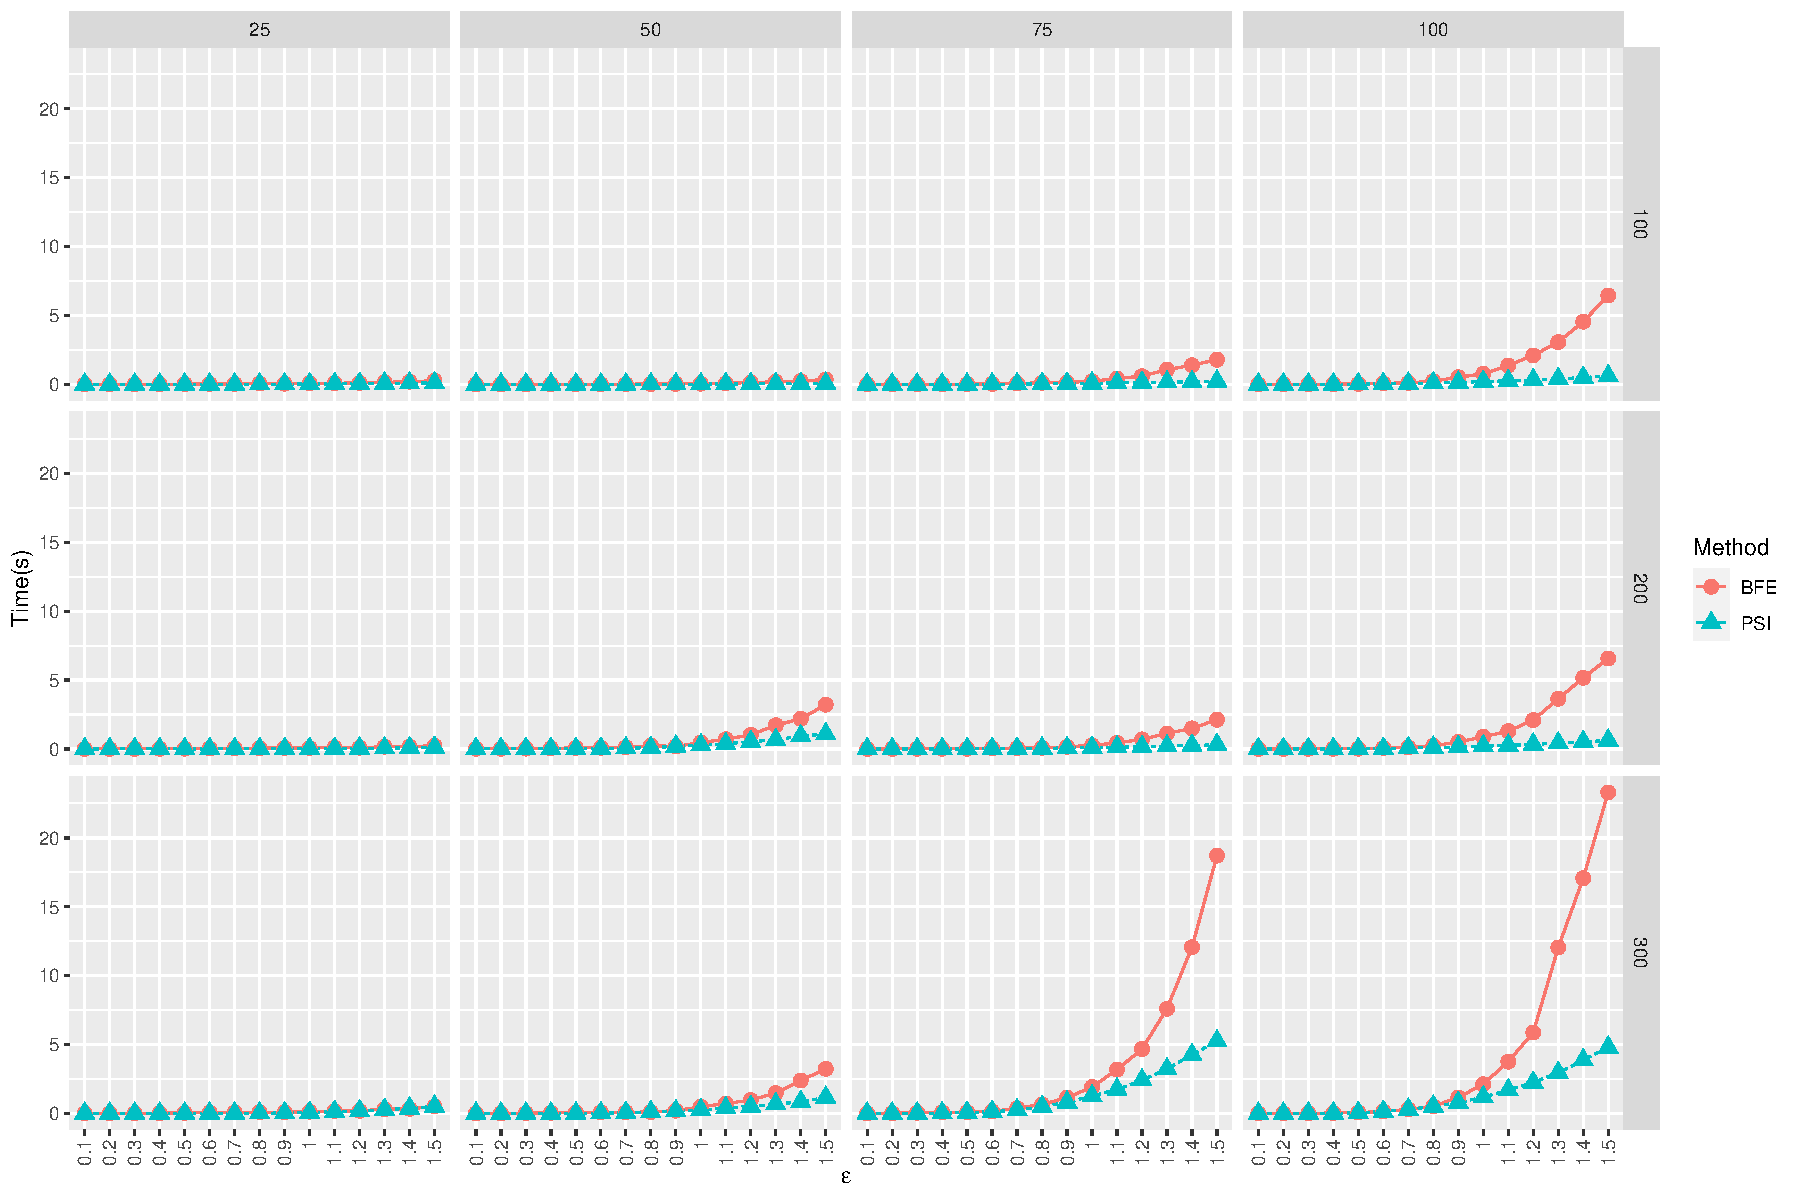
\includegraphics[width=0.95\textwidth]{scripts/uniform_benchmark_lt15}
\end{frame}

\begin{frame}{Performance [Datasets vs Capacity vs Epsilon]...}
    \centering
    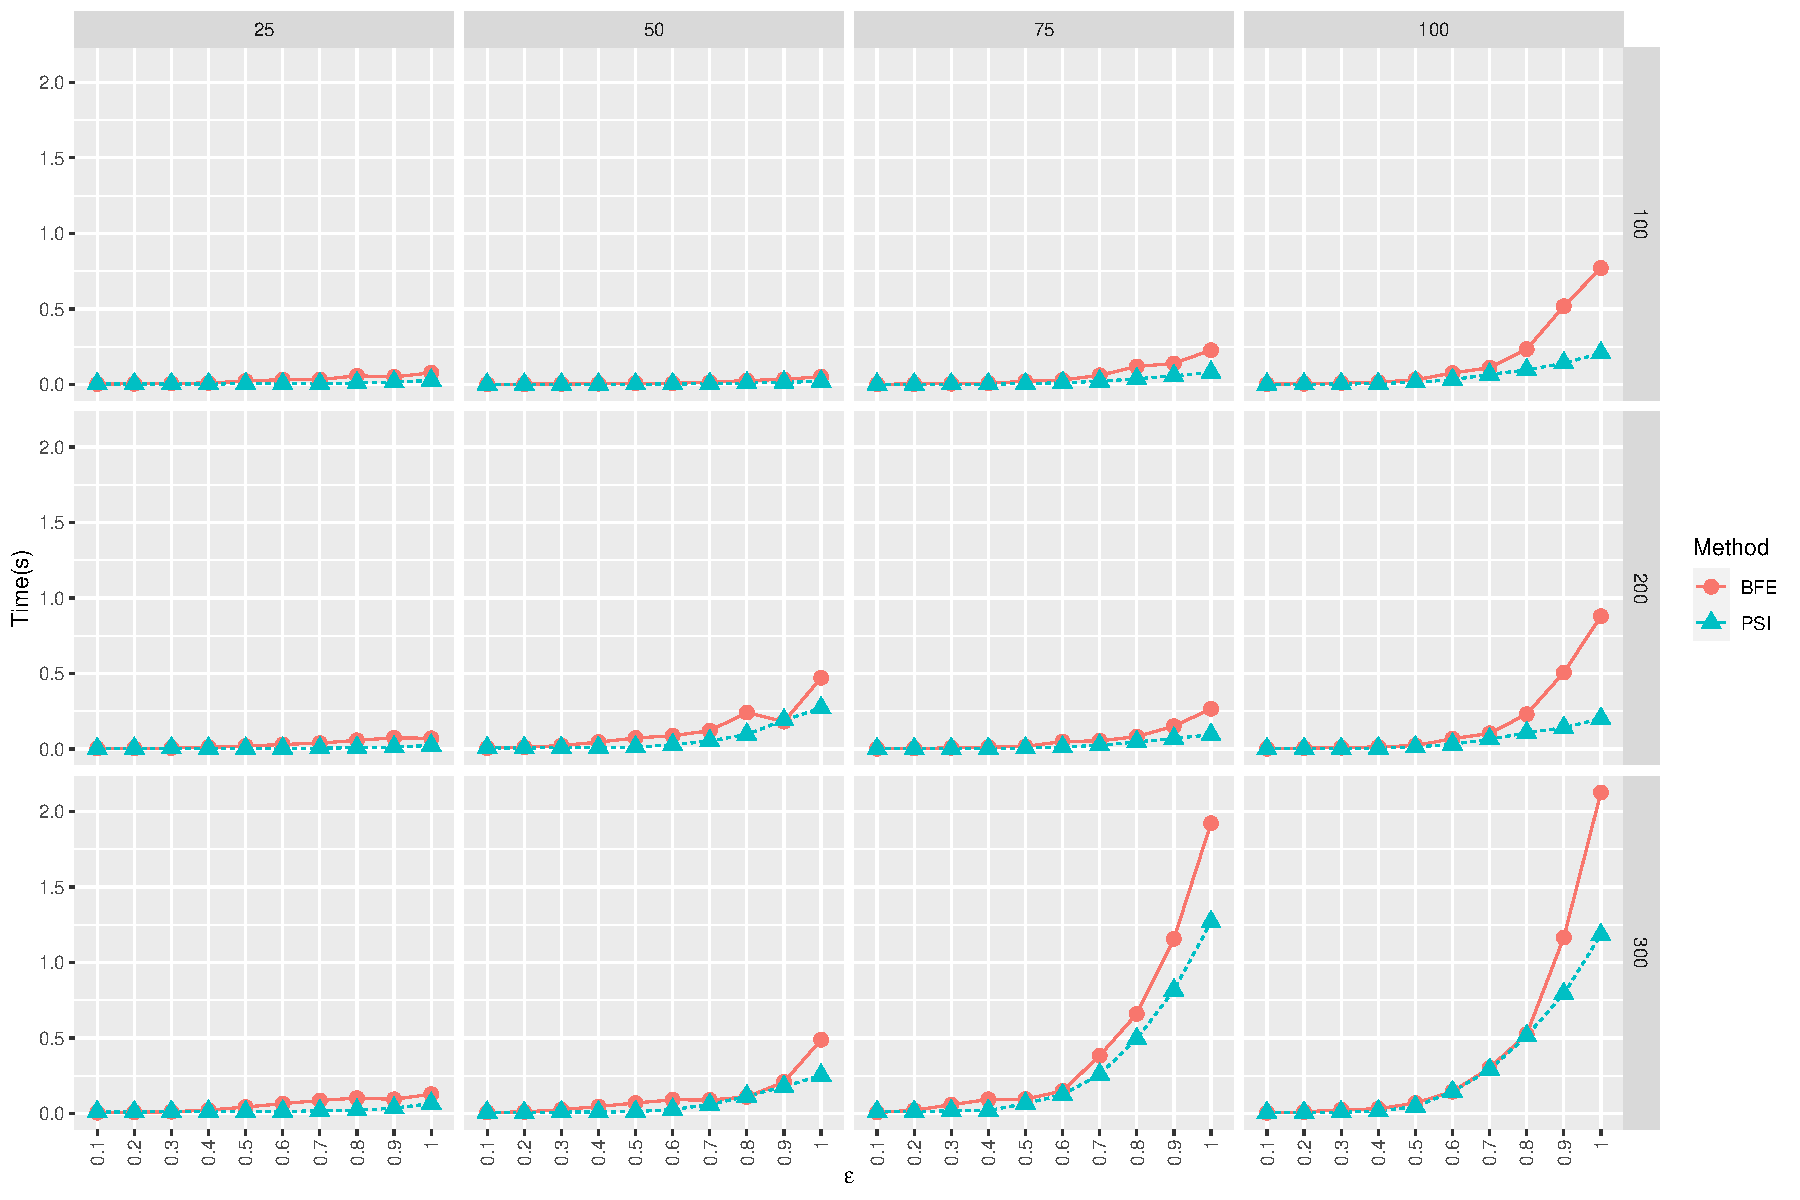
\includegraphics[width=0.95\textwidth]{scripts/uniform_benchmark_lt10}
\end{frame}

\begin{frame}{Performance [Datasets vs Capacity vs Epsilon]...}
    \centering
    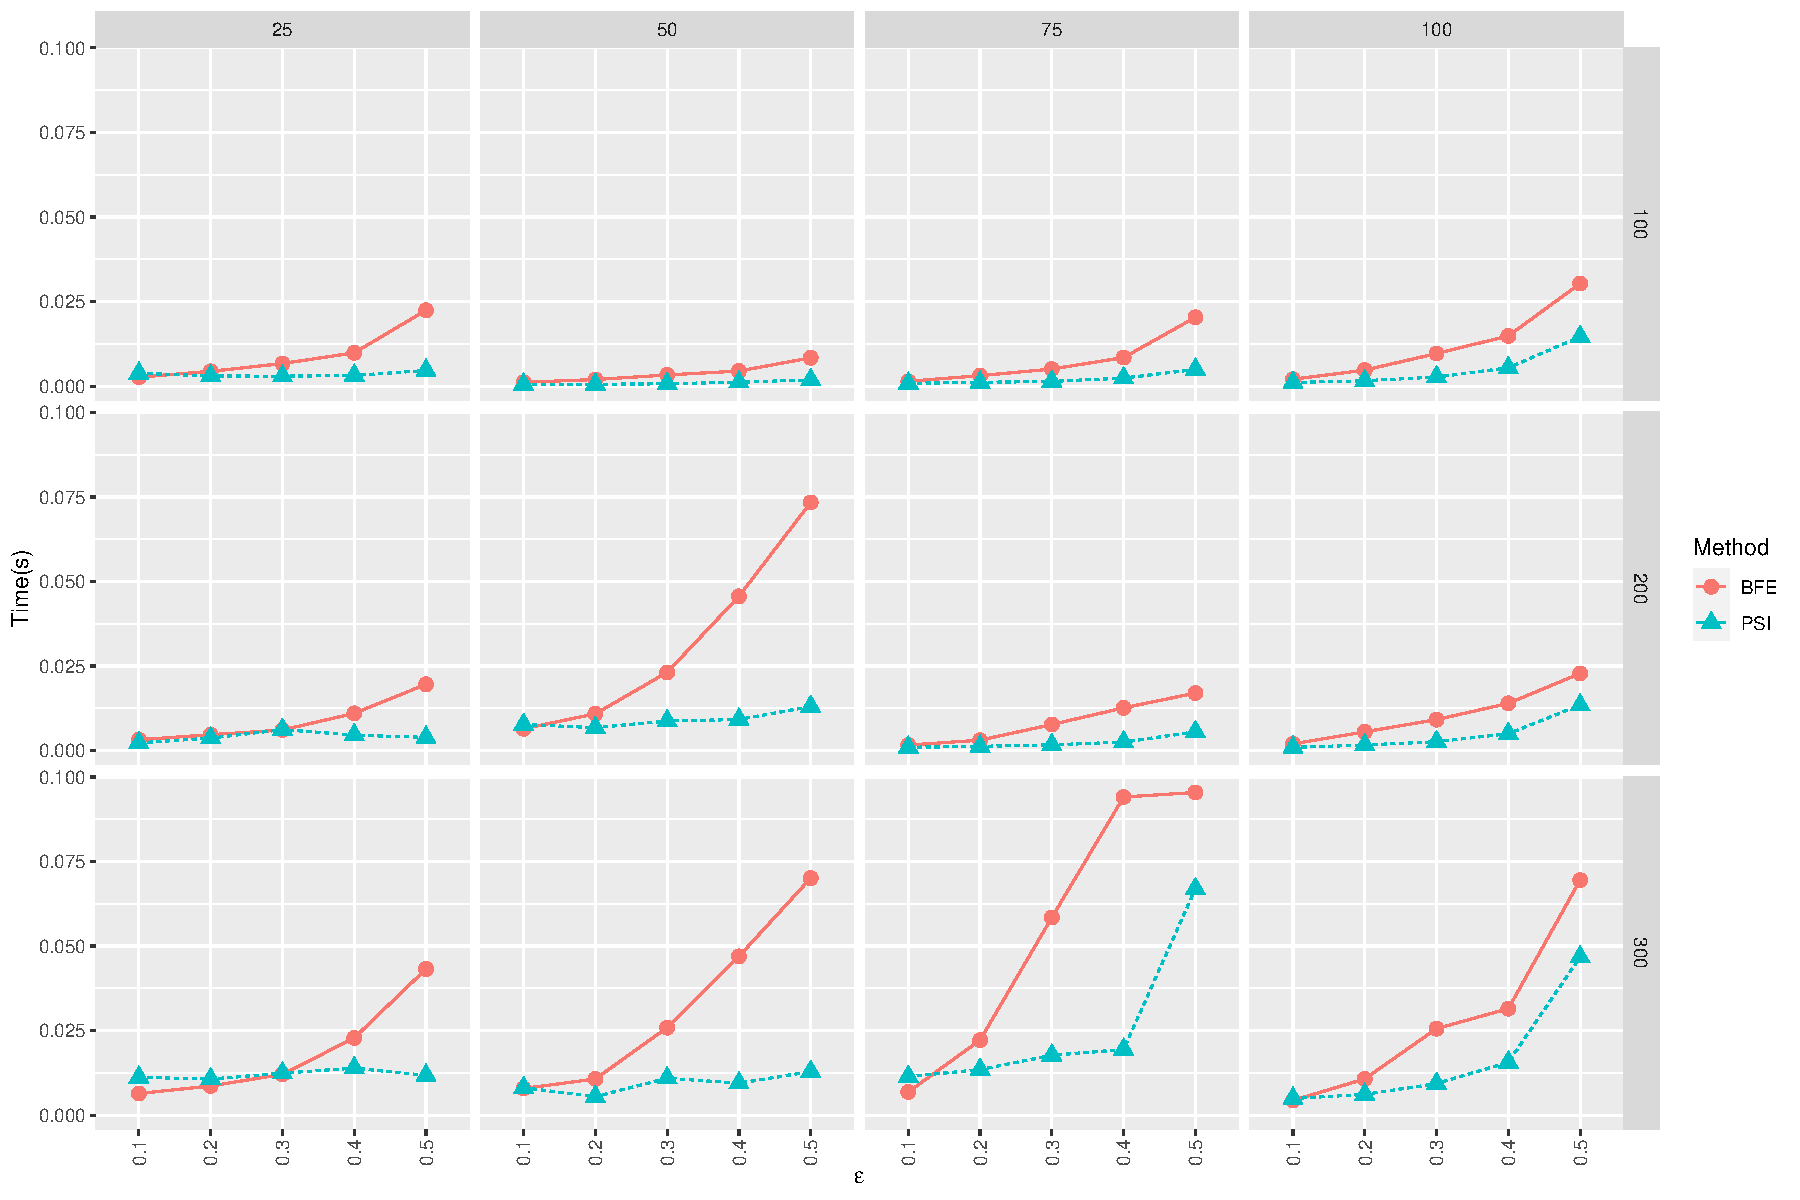
\includegraphics[width=0.95\textwidth]{scripts/uniform_benchmark_lt05}
\end{frame}

\begin{frame}{Uniform study area...}
    \begin{itemize}
        \item Full dataset size: 801M  observations...
        \item California dataset: 59.8M ...
    \end{itemize} \vspace{0.5cm}
    \centering
    \includegraphics[width=0.75\textwidth]{figures/ebird}
\end{frame}

\begin{frame}{eBirds 1\% sample dataset...}
    \centering
    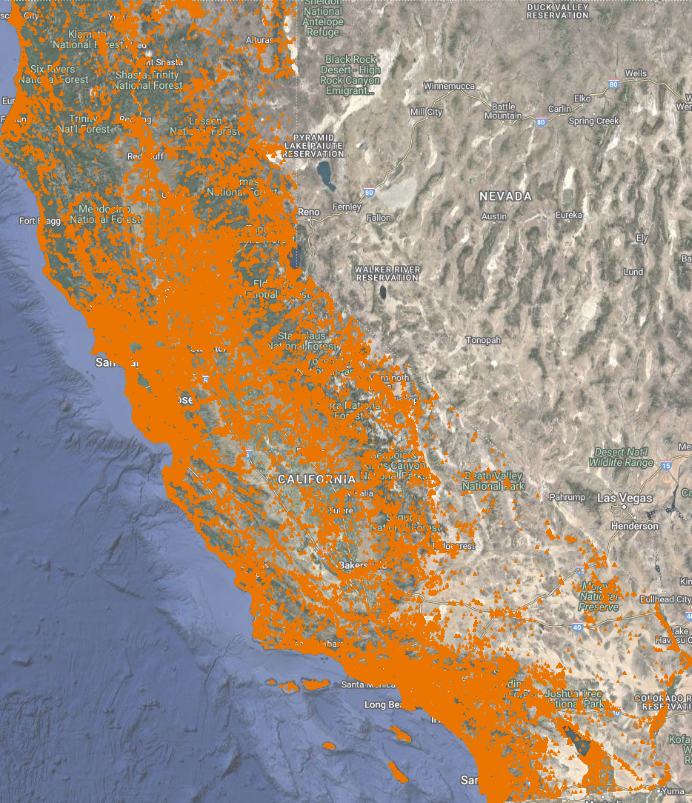
\includegraphics[width=0.5\textwidth]{figures/ebirds_sample_1perc}
\end{frame}
\begin{frame}{eBirds unique spatial locations (450K)...}
    \centering
    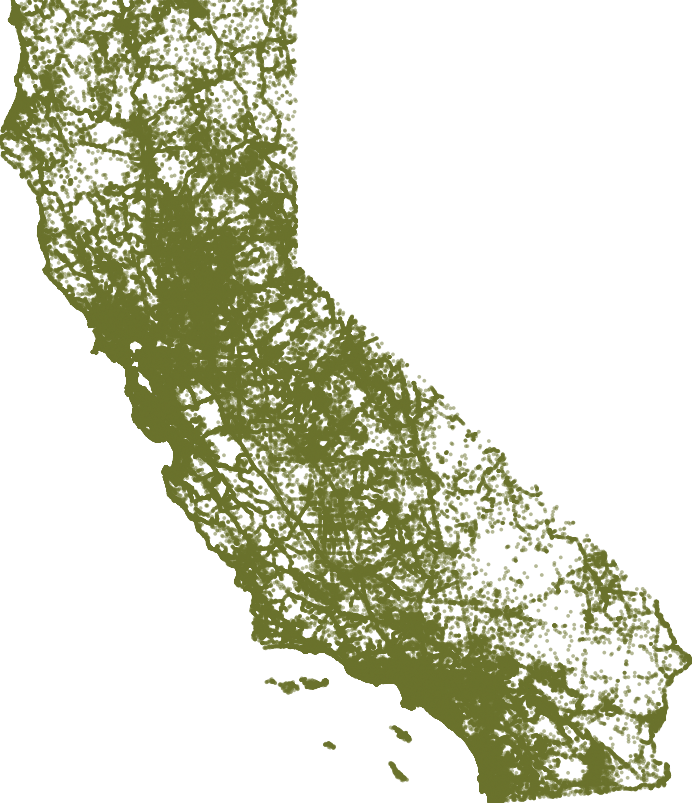
\includegraphics[width=0.5\textwidth]{figures/ebirds_unique_spatial_location}
\end{frame}
\begin{frame}{eBirds unique spatiotemporal locations (3.1M)...}
    \centering
    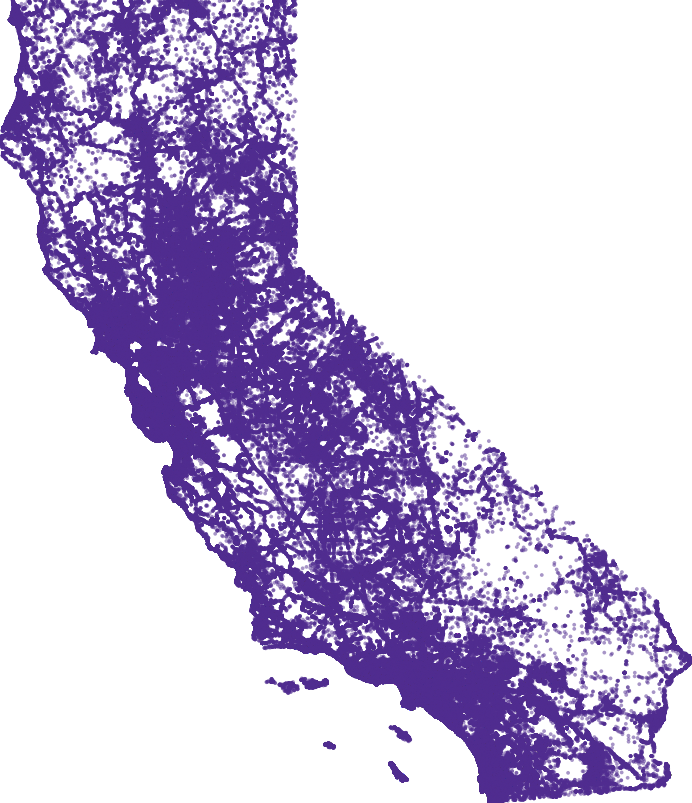
\includegraphics[width=0.5\textwidth]{figures/ebirds_unique_spatiotemporal_location}
\end{frame}
%%%%%%%%%%%%%%%%%%%%%%%%%%%%%%%%%%%%%%%%%%%

\end{document}

